\def\pgfsysdriver{pgfsys-dvisvgm.def}
\documentclass[tikz,border=5pt]{standalone}

\usepackage{tikz-feynman}
\usepackage[fontset=none]{ctex}
\setCJKsansfont[Path=C:/Windows/Fonts/]{NotoSansSC-VF.ttf}

\definecolor{qftink}{HTML}{26363F}
\definecolor{qftmuted}{HTML}{657B85}
\definecolor{qftsakura}{HTML}{D86483}

\tikzfeynmanset{compat=1.1.0}
\tikzset{
  qft scalar/.style={draw=qftink, line width=0.8pt},
  qft vertex/.style={circle, fill=qftsakura, draw=qftsakura,
    inner sep=1.35pt},
  qft counterterm/.style={circle, fill=white, draw=qftsakura,
    line width=0.9pt, inner sep=2.1pt},
  topology label/.style={font=\sffamily\footnotesize, text=qftmuted},
  point label/.style={font=\small, text=qftink},
}

\begin{document}
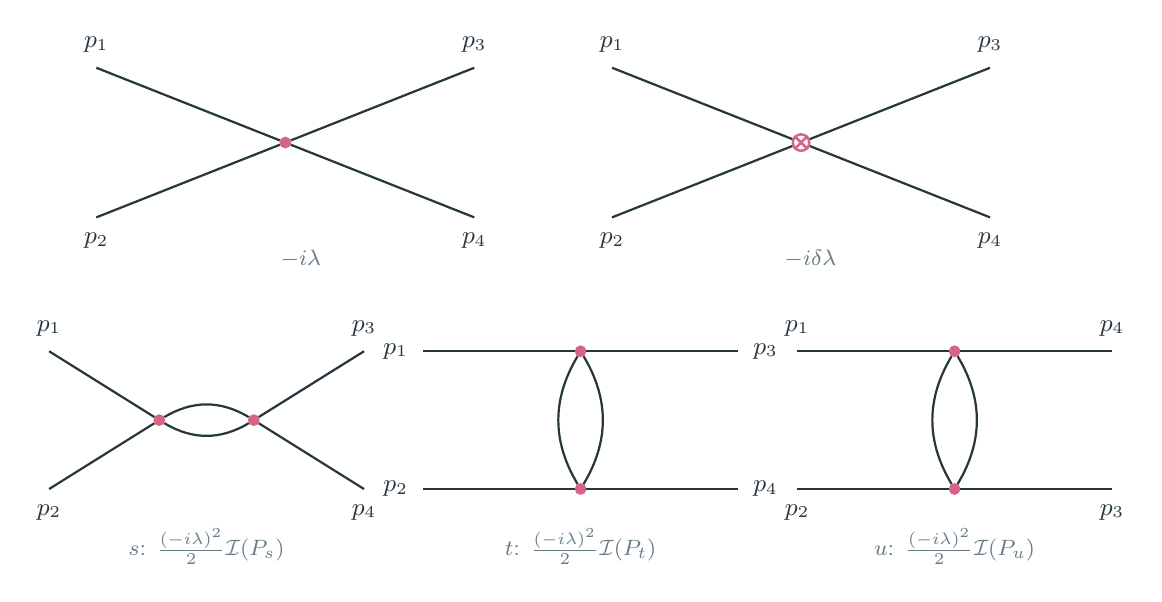
\begin{tikzpicture}[x=1cm, y=1cm]
  % Tree-level contact graph.
  \begin{scope}[shift={(0.55,3.55)}]
    \begin{feynman}
      \vertex (p1) at (0.15,2.35);
      \vertex (p2) at (0.15,0.45);
      \vertex[qft vertex] (z) at (2.55,1.40) {};
      \vertex (p3) at (4.95,2.35);
      \vertex (p4) at (4.95,0.45);
      \diagram*{
        (p1) -- [qft scalar] (z),
        (p2) -- [qft scalar] (z),
        (z) -- [qft scalar] (p3),
        (z) -- [qft scalar] (p4)
      };
    \end{feynman}
    \node[point label, above=2pt] at (p1) {$p_1$};
    \node[point label, below=2pt] at (p2) {$p_2$};
    \node[point label, above=2pt] at (p3) {$p_3$};
    \node[point label, below=2pt] at (p4) {$p_4$};
    \node[topology label] at (2.55,-0.08)
      {树级接触：$-i\lambda$};
  \end{scope}

  % The four-point counterterm is a distinct graph with the same four legs.
  \begin{scope}[shift={(7.10,3.55)}]
    \begin{feynman}
      \vertex (p1) at (0.15,2.35);
      \vertex (p2) at (0.15,0.45);
      \vertex[qft counterterm] (ct) at (2.55,1.40) {};
      \vertex (p3) at (4.95,2.35);
      \vertex (p4) at (4.95,0.45);
      \diagram*{
        (p1) -- [qft scalar] (ct),
        (p2) -- [qft scalar] (ct),
        (ct) -- [qft scalar] (p3),
        (ct) -- [qft scalar] (p4)
      };
    \end{feynman}
    \draw[qftsakura, line width=0.9pt]
      ($(ct)+(-0.085,-0.085)$) -- ($(ct)+(0.085,0.085)$);
    \draw[qftsakura, line width=0.9pt]
      ($(ct)+(-0.085,0.085)$) -- ($(ct)+(0.085,-0.085)$);
    \node[point label, above=2pt] at (p1) {$p_1$};
    \node[point label, below=2pt] at (p2) {$p_2$};
    \node[point label, above=2pt] at (p3) {$p_3$};
    \node[point label, below=2pt] at (p4) {$p_4$};
    \node[topology label] at (2.55,-0.08)
      {反项：$-i\delta\lambda$};
  \end{scope}

  % s-channel fish graph.
  \begin{scope}[shift={(0,0)}]
    \begin{feynman}
      \vertex (p1) at (0.10,2.30);
      \vertex (p2) at (0.10,0.55);
      \vertex[qft vertex] (z1) at (1.50,1.425) {};
      \vertex[qft vertex] (z2) at (2.70,1.425) {};
      \vertex (p3) at (4.10,2.30);
      \vertex (p4) at (4.10,0.55);
      \diagram*{
        (p1) -- [qft scalar] (z1),
        (p2) -- [qft scalar] (z1),
        (z1) -- [qft scalar, bend left=31] (z2),
        (z1) -- [qft scalar, bend right=31] (z2),
        (z2) -- [qft scalar] (p3),
        (z2) -- [qft scalar] (p4)
      };
    \end{feynman}
    \node[point label, above=2pt] at (p1) {$p_1$};
    \node[point label, below=2pt] at (p2) {$p_2$};
    \node[point label, above=2pt] at (p3) {$p_3$};
    \node[point label, below=2pt] at (p4) {$p_4$};
    \node[topology label] at (2.10,-0.18)
      {$s$: $\frac{(-i\lambda)^2}{2}\mathcal I(P_s)$};
  \end{scope}

  % t-channel fish graph.
  \begin{scope}[shift={(4.75,0)}]
    \begin{feynman}
      \vertex (p1) at (0.10,2.30);
      \vertex[qft vertex] (z1) at (2.10,2.30) {};
      \vertex (p3) at (4.10,2.30);
      \vertex (p2) at (0.10,0.55);
      \vertex[qft vertex] (z2) at (2.10,0.55) {};
      \vertex (p4) at (4.10,0.55);
      \diagram*{
        (p1) -- [qft scalar] (z1) -- [qft scalar] (p3),
        (p2) -- [qft scalar] (z2) -- [qft scalar] (p4),
        (z1) -- [qft scalar, bend left=31] (z2),
        (z1) -- [qft scalar, bend right=31] (z2)
      };
    \end{feynman}
    \node[point label, left=2pt] at (p1) {$p_1$};
    \node[point label, left=2pt] at (p2) {$p_2$};
    \node[point label, right=2pt] at (p3) {$p_3$};
    \node[point label, right=2pt] at (p4) {$p_4$};
    \node[topology label] at (2.10,-0.18)
      {$t$: $\frac{(-i\lambda)^2}{2}\mathcal I(P_t)$};
  \end{scope}

  % u-channel fish graph: the outgoing labels are exchanged.
  \begin{scope}[shift={(9.50,0)}]
    \begin{feynman}
      \vertex (p1) at (0.10,2.30);
      \vertex[qft vertex] (z1) at (2.10,2.30) {};
      \vertex (p4) at (4.10,2.30);
      \vertex (p2) at (0.10,0.55);
      \vertex[qft vertex] (z2) at (2.10,0.55) {};
      \vertex (p3) at (4.10,0.55);
      \diagram*{
        (p1) -- [qft scalar] (z1) -- [qft scalar] (p4),
        (p2) -- [qft scalar] (z2) -- [qft scalar] (p3),
        (z1) -- [qft scalar, bend left=31] (z2),
        (z1) -- [qft scalar, bend right=31] (z2)
      };
    \end{feynman}
    \node[point label, above=2pt] at (p1) {$p_1$};
    \node[point label, below=2pt] at (p2) {$p_2$};
    \node[point label, above=2pt] at (p4) {$p_4$};
    \node[point label, below=2pt] at (p3) {$p_3$};
    \node[topology label] at (2.10,-0.18)
      {$u$: $\frac{(-i\lambda)^2}{2}\mathcal I(P_u)$};
  \end{scope}
\end{tikzpicture}
\end{document}
